\begin{center}
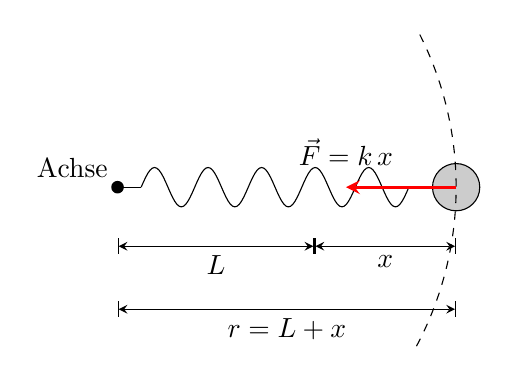
\begin{tikzpicture}[>=stealth]
 \fill (0,0) circle (0.08) node[above left] {Achse};
 \draw (0,0) -- (0.3,0);
 \draw[domain=0.3:3.7, samples=121] plot (\x, {0.25*sin(1800*(\x-0.3)/3.4)});
 \draw (3.7,0) -- (4.0,0);
 \draw[fill=gray!40] (4.3,0) circle (0.3);
 \draw[dashed] (0,0) ++(-28:4.3) arc (-28:28:4.3);
 \draw[->, very thick, red] (4.3,0) -- (2.9,0) node[above=4pt, black] {$\vec F = k\,x$};
 \draw[|<->|] (0,-0.75) -- (2.5,-0.75) node[midway, below] {$L$};
 \draw[|<->|] (2.5,-0.75) -- (4.3,-0.75) node[midway, below] {$x$};
 \draw[|<->|] (0,-1.55) -- (4.3,-1.55) node[midway, below] {$r = L + x$};
\end{tikzpicture}
\end{center}

Die Kugel bewegt sich auf einem Kreis mit dem Radius $r = L + x$, wobei $x$ die gesuchte Dehnung ist. Die Federkraft $k\,x$ liefert die Zentripetalkraft:
\begin{align}
 k\,x &= m\,\omega^2\left(L + x\right) \quad\text{mit}\quad \omega = 2\pi f
\end{align}
Nach $x$ aufgelöst:
\begin{align}
 x\left(k - m\,\omega^2\right) &= m\,\omega^2 L \\
 x &= \xFeF \\
   &= \frac{\mFe\cdot\left(2\pi\cdot\fFe\right)^2\cdot\LFe}{\kFe-\mFe\cdot\left(2\pi\cdot\fFe\right)^2} \\
   &= \xFe \approx \result{\xFeP{-2}{2}}
\end{align}
Eine Gleichgewichtslage gibt es nur, solange $m\,\omega^2 < k$ ist, also für
\begin{align}
 f &< \fFemaxF = \fFemaxP{0}{2}
\end{align}
Bei höherer Frequenz kann die Feder die nötige Zentripetalkraft nicht aufbringen: Je mehr sie sich dehnt, desto grösser wird auch der Radius und damit die benötigte Kraft, und die Feder wird immer weiter gedehnt.
